% Provenance (never printed): see sources/outline_sources.md (Year 3:
% atmospheric dynamics: vorticity and potential vorticity, Rossby waves,
% baroclinic instability, the general circulation and the Hadley cell).
% Brief: sources/book5/BRIEFS.md, ch. 20. Curves from
% figdata/bachelor-3/rossby_waves.py, eady.py and held_hou.py. Exercise and
% problem values in the Book 5 scratch calculator calc/ch20.py. The waves,
% shears and parcels of the exercises and the problem are invented.
\chapter{Atmospheric Dynamics}\label{ch:b3:atmospheric-dynamics}

On a winter map of the upper troposphere the jet stream does not circle the
pole as a smooth ring. It meanders, in a few great waves round the
hemisphere, troughs reaching towards the subtropics and ridges towards the
pole, and at the surface depressions are born, grow for a few days and die
under them. The waves drift slowly, sometimes against the wind that carries
them. Their number, their speed and the growth of the storms beneath them
follow from one conserved quantity, the vorticity of the air seen from
space, and from the energy stored in the temperature contrast between the
tropics and the poles.

\begin{recall}
Vorticity and circulation are in the physics books. The Rossby waves of the
upper troposphere, troughs and ridges, the extratropical cyclone and the
principle of numerical weather prediction are described in the Year~2
volume, in its chapter on weather systems. The Hadley, Ferrel and polar
cells, the jets, the westerlies and the angular-momentum wind of a ring of
air are in the Year~1 volume, in its chapter on the general circulation of
the atmosphere, and the poleward transport of heat in its chapter on
radiation and heat transport. The Coriolis parameter $f$, the $\beta$-plane,
the Rossby radius and the \omterm{thm:b3:gfd-foundations:thermal-wind}{thermal wind} are in
Chapter~\ref{ch:b3:gfd-foundations}.
\end{recall}

\section{Vorticity}\label{sec:b3:atmospheric-dynamics:vorticity}

The vorticity of a fluid, the curl of its velocity, is twice its local
angular velocity. For the large-scale atmosphere only its vertical
component matters, and the rotation of the Earth contributes to it.

\begin{definition}[Relative, planetary and absolute vorticity]\label{def:b3:atmospheric-dynamics:vorticity-kinds}
For a horizontal velocity $(u, v)$, the \emph{relative
vorticity}\index{relative vorticity} is the vertical component of the curl
of the velocity relative to the ground, $\zeta = \partial v/\partial x -
\partial u/\partial y$, positive for anticlockwise rotation seen from above.
The \emph{planetary vorticity}\index{planetary vorticity} is the vertical
component of the vorticity of the Earth's rotation, $2\Omega\sin\varphi =
f$. The \emph{absolute vorticity}\index{absolute vorticity} is their sum,
$\zeta + f$.
\end{definition}

In the Northern Hemisphere a depression, where the air turns anticlockwise,
has $\zeta > 0$ and is called cyclonic; an anticyclone has $\zeta < 0$. A
wind of \qty{15}{m/s} turning on a circle of \qty{1000}{km} has $\zeta =
2V/R = \qty{3e-5}{s^{-1}}$ in solid rotation, a third of $f$ at \ang{45}:
the planetary part is usually the larger.

\begin{theorem}[Barotropic vorticity equation]\label{thm:b3:atmospheric-dynamics:bve}
In an inviscid, two-dimensional flow without horizontal divergence on a
$\beta$-plane, the \omterm{def:b3:atmospheric-dynamics:vorticity-kinds}{absolute vorticity} of each parcel is conserved:
\[
\frac{\mathrm D(\zeta + f)}{\mathrm Dt} = 0 ,
\qquad\text{that is}\qquad
\frac{\partial\zeta}{\partial t} + u\frac{\partial\zeta}{\partial x} + v\frac{\partial\zeta}{\partial y} + \beta v = 0 .
\]
This is the \emph{barotropic vorticity equation}\index{barotropic vorticity equation}.
\end{theorem}

\begin{proof}
The horizontal momentum equations are $\mathrm Du/\mathrm Dt - fv =
-(1/\rho_0)\partial p/\partial x$ and $\mathrm Dv/\mathrm Dt + fu =
-(1/\rho_0)\partial p/\partial y$. Differentiate the second with respect to
$x$, the first with respect to $y$, and subtract: the pressure disappears.
With $\delta = \partial u/\partial x + \partial v/\partial y$, the
advective terms give $\partial_x(u\,\partial_xv + v\,\partial_yv) -
\partial_y(u\,\partial_xu + v\,\partial_yu) = u\,\partial_x\zeta +
v\,\partial_y\zeta + \zeta\delta$, and the Coriolis terms $f\delta + \beta
v$. Hence $\mathrm D\zeta/\mathrm Dt + \beta v = -(\zeta + f)\,\delta$. For
$\delta = 0$, and since $\mathrm Df/\mathrm Dt = \beta v$, $\mathrm D(\zeta +
f)/\mathrm Dt = 0$.
\end{proof}

The proof also gave the general law, $\mathrm D(\zeta + f)/\mathrm Dt =
-(\zeta + f)\delta$: convergence spins a column up, divergence spins it
down, like a skater pulling in or spreading her arms. In a layer whose
depth changes, convergence is tied to the stretching of the column, and
the conserved quantity becomes a ratio.

\begin{definition}[Potential vorticity]\label{def:b3:atmospheric-dynamics:pv}
The \emph{potential vorticity}\index{potential vorticity} of a column of a
homogeneous layer of depth $h$ is $q = (\zeta + f)/h$. In a continuously
stratified fluid, Ertel's potential vorticity is $q = (\vec\omega_a\cdot
\nabla\theta)/\rho$, with $\vec\omega_a$ the \omterm{def:b3:atmospheric-dynamics:vorticity-kinds}{absolute vorticity} vector and
$\theta$ the potential temperature.
\end{definition}

\begin{theorem}[Conservation of potential vorticity]\label{thm:b3:atmospheric-dynamics:pv}
In a homogeneous, hydrostatic, inviscid layer of variable depth $h$ whose
horizontal velocity does not vary with height, $\mathrm Dq/\mathrm Dt = 0$
for $q = (\zeta + f)/h$.
\end{theorem}

\begin{proof}
From the proof above, $\mathrm D(\zeta + f)/\mathrm Dt = -(\zeta + f)\delta$.
Mass conservation in a column of uniform density gives $\mathrm Dh/\mathrm
Dt = -h\delta$. Then $\mathrm Dq/\mathrm Dt = (1/h)\,\mathrm D(\zeta +
f)/\mathrm Dt - ((\zeta + f)/h^2)\,\mathrm Dh/\mathrm Dt = -(\zeta +
f)\delta/h + (\zeta + f)\delta/h = 0$.
\end{proof}

Ertel's form is conserved in the same way by an adiabatic, frictionless
flow of a stratified fluid, with the distance between two surfaces of
constant $\theta$ playing the part of $h$. A column of air crossing a
mountain range is squeezed on the way up: its \omterm{def:b3:atmospheric-dynamics:vorticity-kinds}{absolute vorticity} falls, it
turns anticyclonically over the crest, and it stretches and turns
cyclonically in the lee. Conservation of
absolute or \omterm{def:b3:atmospheric-dynamics:pv}{potential vorticity} is the restoring mechanism of the waves
of the next section, as the figure below shows.

\begin{omfigure}
\begin{tikzpicture}[>=stealth, font=\small, declare function={w(\x)=0.9*sin(\x r);}]
\draw[black!40, dashed] (0,0) -- (12.6,0) node[right, font=\scriptsize] {latitude $\varphi_0$};
\draw[thick, omDef, domain=0:12.566, samples=120] plot (\x, {w(\x)});
\foreach \x in {0.785, 2.356, 3.927, 5.498, 7.069, 8.639, 10.21, 11.78}
  \fill (\x, {w(\x)}) circle (0.06);
% crests: clockwise (anticyclonic), troughs: anticlockwise (cyclonic)
\foreach \x in {1.571, 7.854} {
  \draw[->, omThm, thick] (\x+0.45,{w(\x)+0.05}) arc (0:-300:0.45);
  \node[font=\scriptsize, omThm] at (\x,{w(\x)+0.75}) {$\zeta < 0$};}
\foreach \x in {4.712, 10.996} {
  \draw[->, omMeth, thick] (\x+0.45,{w(\x)-0.05}) arc (0:300:0.45);
  \node[font=\scriptsize, omMeth] at (\x,{w(\x)-0.75}) {$\zeta > 0$};}
\foreach \x in {3.1416, 9.4248} \draw[->, very thick] (\x,0.45) -- (\x,-0.45);
\foreach \x in {6.2832} \draw[->, very thick] (\x,-0.45) -- (\x,0.45);
\draw[->, thick] (8.4,-2.25) -- (6.4,-2.25) node[left, font=\scriptsize] {the pattern moves west};
\draw[->] (0,-2.25) -- (1.4,-2.25) node[right, font=\scriptsize] {east};
\draw[->] (0,-2.25) -- (0,-1.65) node[above, font=\scriptsize] {north};
\end{tikzpicture}

\par\smallskip{\small How a Rossby wave moves (schematic, Northern
Hemisphere). A chain of parcels at rest at latitude $\varphi_0$ is
displaced into a wave. Keeping $\zeta + f$, the parcels moved north, where
$f$ is larger, acquire clockwise \omterm{def:b3:atmospheric-dynamics:vorticity-kinds}{relative vorticity}; those moved south,
anticlockwise. Between a crest and the trough to its east the induced flow
is southward, between a trough and the crest to its east northward (black
arrows): the displacement grows west of each crest and the whole pattern
shifts westward.}\label{fig:b3:atmospheric-dynamics:restoring}
\end{omfigure}

\section{Rossby waves}\label{sec:b3:atmospheric-dynamics:rossby}

The Year~2 volume described the Rossby waves of the upper troposphere. The
\omterm{thm:b3:atmospheric-dynamics:bve}{barotropic vorticity equation} explains them. Write the flow as a uniform
westerly $U$ plus a small disturbance with streamfunction $\psi'$, so that
$u' = -\partial\psi'/\partial y$, $v' = \partial\psi'/\partial x$ and $\zeta'
= \nabla^2\psi'$.

\begin{theorem}[Dispersion of Rossby waves]\label{thm:b3:atmospheric-dynamics:rossby}
Small disturbances $\psi' \propto \mathrm e^{\mathrm i(kx + ly - \omega t)}$
of a uniform westerly $U$ on a $\beta$-plane obey the
\emph{Rossby-wave dispersion relation}\index{Rossby-wave dispersion relation}
\[
\omega = Uk - \frac{\beta k}{k^2 + l^2} .
\]
Their eastward phase speed is $c = \omega/k = U - \beta/K^2$, with $K^2 =
k^2 + l^2$, and their eastward group velocity $c_g = \partial\omega/\partial
k = U + \beta(k^2 - l^2)/K^4$.
\end{theorem}

\begin{proof}
Linearised about $U$, the \omterm{thm:b3:atmospheric-dynamics:bve}{barotropic vorticity equation} reads
$(\partial_t + U\partial_x)\nabla^2\psi' + \beta\,\partial_x\psi' = 0$, the
products of small quantities being dropped and $\zeta$ of the basic flow
being zero. For the plane wave, $\partial_t \to -\mathrm i\omega$,
$\partial_x \to \mathrm ik$ and $\nabla^2 \to -K^2$: $(-\mathrm i\omega +
\mathrm iUk)(-K^2) + \mathrm i\beta k = 0$, that is $(\omega - Uk)K^2 =
-\beta k$. Differentiating $\omega$ with respect to $k$ gives $c_g = U -
\beta/K^2 + 2\beta k^2/K^4$, which is the stated form.
\end{proof}

\begin{omfigure}
\begin{tikzpicture}
\begin{groupplot}[group style={group size=2 by 1, horizontal sep=1.7cm},
  width=0.48\linewidth, height=0.46\linewidth, tick label style={font=\scriptsize},
  label style={font=\small}, legend style={font=\scriptsize, draw=none, fill=none}]
\nextgroupplot[xlabel={zonal wavenumber $n$}, ylabel={speed (\unit{m/s})},
  xmin=1, xmax=12, ymin=-40, ymax=60, legend pos=north east, legend cell align=left,
  title={\small \ang{45} N}]
% computed in figdata/bachelor-3/rossby_waves.py
\addplot[omThm, thick] table[x=n, y=c15] {figdata/out/bachelor-3-rossby_waves-disp.dat};
\addlegendentry{$c$, $U = 15$}
\addplot[omThm, thick, densely dashed] table[x=n, y=cg15] {figdata/out/bachelor-3-rossby_waves-disp.dat};
\addlegendentry{$c_g$, $U = 15$}
\addplot[omDef, thick] table[x=n, y=c0] {figdata/out/bachelor-3-rossby_waves-disp.dat};
\addlegendentry{$c$, $U = 0$}
\addplot[omDef, thick, densely dashed] table[x=n, y=cg0] {figdata/out/bachelor-3-rossby_waves-disp.dat};
\addlegendentry{$c_g$, $U = 0$}
\addplot[black!50, thin, domain=1:12, samples=2, forget plot] {0};
\nextgroupplot[xlabel={latitude (\unit{\degree} N)}, ylabel={stationary wavenumber $n_s$},
  xmin=20, xmax=75, ymin=0, ymax=9, legend pos=north east, legend cell align=left]
\addplot[omMeth, thick] table[x=lat, y=n10] {figdata/out/bachelor-3-rossby_waves-stat.dat};
\addplot[omDef, thick] table[x=lat, y=n15] {figdata/out/bachelor-3-rossby_waves-stat.dat};
\addplot[omThm, thick] table[x=lat, y=n20] {figdata/out/bachelor-3-rossby_waves-stat.dat};
\addplot[black, only marks, mark=*, mark size=1.1pt] table[x=lat, y=ns] {figdata/out/bachelor-3-rossby_waves-statobs.dat};
\legend{\qty{10}{m/s}, \qty{15}{m/s}, \qty{20}{m/s}, January \qty{300}{hPa}}
\end{groupplot}
\end{tikzpicture}

\par\smallskip{\small Left, the eastward phase speed $c$ (solid) and group
velocity $c_g$ (dashed) of Rossby waves with $l = 0$ at \ang{45} N, against
the number of waves round the latitude circle, without a mean wind (blue)
and in a westerly of \qty{15}{m/s} (red): long waves move west, short ones
are carried east, and $c_g > c$. Right, the stationary wavenumber for
uniform westerlies of 10, 15 and \qty{20}{m/s}, and for the January
zonal-mean wind at \qty{300}{hPa} of each latitude (dots, NCEP--NCAR
Reanalysis~1, 1991--2020).}\label{fig:b3:atmospheric-dynamics:rossby}
\end{omfigure}
% ledger: data:b5-ncep-uwnd, geod5:grs80-defining, earth:Rmean

Relative to the air, the waves always move west, the faster the longer
they are. A westerly wind carries the short waves east; the long ones it
cannot carry, and they drift west against it. In between, one length
stands still.

\begin{proposition}[Stationary Rossby waves]\label{prop:b3:atmospheric-dynamics:stationary}
In a westerly $U > 0$, a wave with no meridional structure ($l = 0$) is
stationary when its wavelength is the \emph{stationary Rossby
wavelength}\index{stationary Rossby wavelength} $\lambda_s =
2\pi\sqrt{U/\beta}$. Round the latitude circle $\varphi$ this is a whole
number of waves close to $n_s = \sqrt{2\Omega a\cos^3\varphi/U}$.
\end{proposition}

\begin{proof}
$c = 0$ when $k^2 = \beta/U$, so $\lambda_s = 2\pi/k = 2\pi\sqrt{U/\beta}$.
The circle has length $2\pi a\cos\varphi$, so $n_s = a\cos\varphi\,k =
a\cos\varphi\sqrt{2\Omega\cos\varphi/(aU)} = \sqrt{2\Omega a\cos^3\varphi/U}$.
\end{proof}

At \ang{45} N in a westerly of \qty{15}{m/s}, with $\beta =
\qty{1.62e-11}{m^{-1}.s^{-1}}$, $\lambda_s = \qty{6050}{km}$ and $n_s =
4.7$: four or five waves round the hemisphere. With the zonal-mean
January wind at \qty{300}{hPa}, about \qty{21}{m/s} at \ang{45} N, $n_s$ is
about four from \ang{35} to \ang{55} N, falling poleward. The group velocity
of a wave with $l = 0$ exceeds its phase speed by $2\beta/k^2$: energy runs
ahead of the wave, so a disturbance set off at one place builds new troughs
and ridges downstream of it, a few days later and thousands of kilometres
east, while the pattern itself barely moves. Mountain ranges and the
contrasts of temperature between continents and oceans force stationary
waves of exactly this kind, through the stretching and squeezing of
\omterm{def:b3:atmospheric-dynamics:pv}{potential vorticity}.
% ledger: geod5:grs80-defining, earth:Rmean, data:b5-ncep-uwnd (values in figdata/bachelor-3/rossby_waves.py)


\section{Baroclinic instability}\label{sec:b3:atmospheric-dynamics:baroclinic}

The waves of the last section are neutral: they neither grow nor decay.
The storms of the middle latitudes grow, and draw their energy from the
temperature contrast that the \omterm{thm:b3:gfd-foundations:thermal-wind}{thermal wind} expresses.

\begin{definition}[Available potential energy]\label{def:b3:atmospheric-dynamics:ape}
The \emph{available potential energy}\index{available potential energy} of
a stratified fluid is the difference between its total potential energy
(gravitational and internal) and the smallest total potential energy it
could reach by an adiabatic rearrangement of its mass, the state in which
the surfaces of constant potential temperature, or potential density, are
horizontal.
\end{definition}

A fluid with horizontal isentropes has none, however much potential energy
it holds; a fluid whose isentropes slope, warm and light on one side, cold
and dense on the other, can release some by letting them slump. Exchanging
two parcels shows how. Take a warm parcel low on the equatorward side and a
cold one high on the poleward side, both on the same isentrope in a stable
atmosphere whose isentropes rise towards the pole. Swapping them along the
isentrope changes nothing. Swapping them along a path less steep than the
isentrope brings the warm parcel up and poleward into air colder than
itself, and the cold parcel down and equatorward into warmer air: the warm
rises, the cold sinks, the centre of mass falls, and kinetic energy is
released. Paths inside this wedge between the horizontal and the
isentropes release energy; the eddies of the middle latitudes are such
exchanges, moving heat poleward and upward.

\begin{definition}[Baroclinic instability]\label{def:b3:atmospheric-dynamics:baroclinic-instability}
\emph{Baroclinic instability}\index{baroclinic instability} is the
instability of a rotating, stratified flow in thermal-wind balance, through
which disturbances grow by converting the \omterm{def:b3:atmospheric-dynamics:ape}{available potential energy} of the
sloping isentropes into their own kinetic energy.
\end{definition}

\begin{definition}[Eady model]\label{def:b3:atmospheric-dynamics:eady}
The \emph{Eady model}\index{Eady model} is a Boussinesq fluid on an
$f$-plane between two rigid horizontal surfaces at $z = 0$ and $z = H$, with
uniform \omterm{def:b3:gfd-foundations:buoyancy}{buoyancy frequency} $N$ and a westerly wind that increases linearly
with height, $U = \Lambda z$, in thermal-wind balance with a uniform
poleward decrease of temperature; its disturbances obey the
quasi-geostrophic equations.
\end{definition}

\begin{theorem}[Eady growth rate]\label{thm:b3:atmospheric-dynamics:eady}
In the \omterm{def:b3:atmospheric-dynamics:eady}{Eady model}, disturbances $\propto \mathrm e^{\mathrm ik(x - ct)}$
with $\mu = kL_d$, $L_d = NH/f$, grow exponentially when $\mu < \mu_c =
2.40$, at the rate
\[
\sigma = \frac{f\Lambda}{N}\left[\left(\coth\frac{\mu}{2} - \frac{\mu}{2}\right)\left(\frac{\mu}{2} - \tanh\frac{\mu}{2}\right)\right]^{1/2} .
\]
The fastest-growing disturbance has $\mu = 1.61$, the wavelength $2\pi L_d/1.61
\approx 3.9\,L_d$, and grows at $\sigma_{\max} = 0.31\,f\Lambda/N$.
\end{theorem}
\admitted

The growth rate depends only on the shear and the stratification, through
$f\Lambda/N$, and the preferred size only on the Rossby radius. For the
January mean at \ang{45} N the wind grows by \qty{17.2}{m/s} between
\qty{850}{hPa} and \qty{250}{hPa}, about \qty{8.9}{km} apart in the
standard atmosphere, a shear of \qty{1.9e-3}{s^{-1}}; with the mean
tropospheric $N = \qty{0.0113}{s^{-1}}$ and $H = \qty{11}{km}$, $L_d =
\qty{1210}{km}$, the fastest disturbance has a wavelength of \qty{4700}{km}
and grows by a factor $e$ in \num{2.1}~days. Disturbances shorter than
\qty{3200}{km} do not grow at all. These are the size and the growing time of
the depressions on a weather map.
% ledger: data:b5-ncep-uwnd, nasa:grc-atmos (values in figdata/bachelor-3/eady.py)

\begin{omfigure}
\begin{minipage}[c]{0.52\linewidth}\centering
\begin{tikzpicture}
\begin{axis}[width=\linewidth, height=0.85\linewidth, xmin=2, xmax=16, ymin=0, ymax=0.55,
  xlabel={wavelength (\qty{1000}{km})}, ylabel={growth rate (day$^{-1}$)},
  tick label style={font=\scriptsize}, label style={font=\small}]
% computed in figdata/bachelor-3/eady.py
\addplot[omThm, thick] table[x expr=\thisrow{lam}/1000, y=sday] {figdata/out/bachelor-3-eady-curve.dat};
\addplot[only marks, mark=*, mark size=1.6pt] coordinates {(4.721,0.4701)};
\node[font=\scriptsize, anchor=west] at (axis cs:5.0,0.49) {\qty{4700}{km}: $e$-folding \qty{2.1}{d}};
\addplot[black!50, densely dashed] coordinates {(3.160,0) (3.160,0.55)};
\node[font=\scriptsize, anchor=west, black!60] at (axis cs:3.25,0.04) {cut-off};
\end{axis}
\end{tikzpicture}
\end{minipage}\hfill
\begin{minipage}[c]{0.44\linewidth}\centering
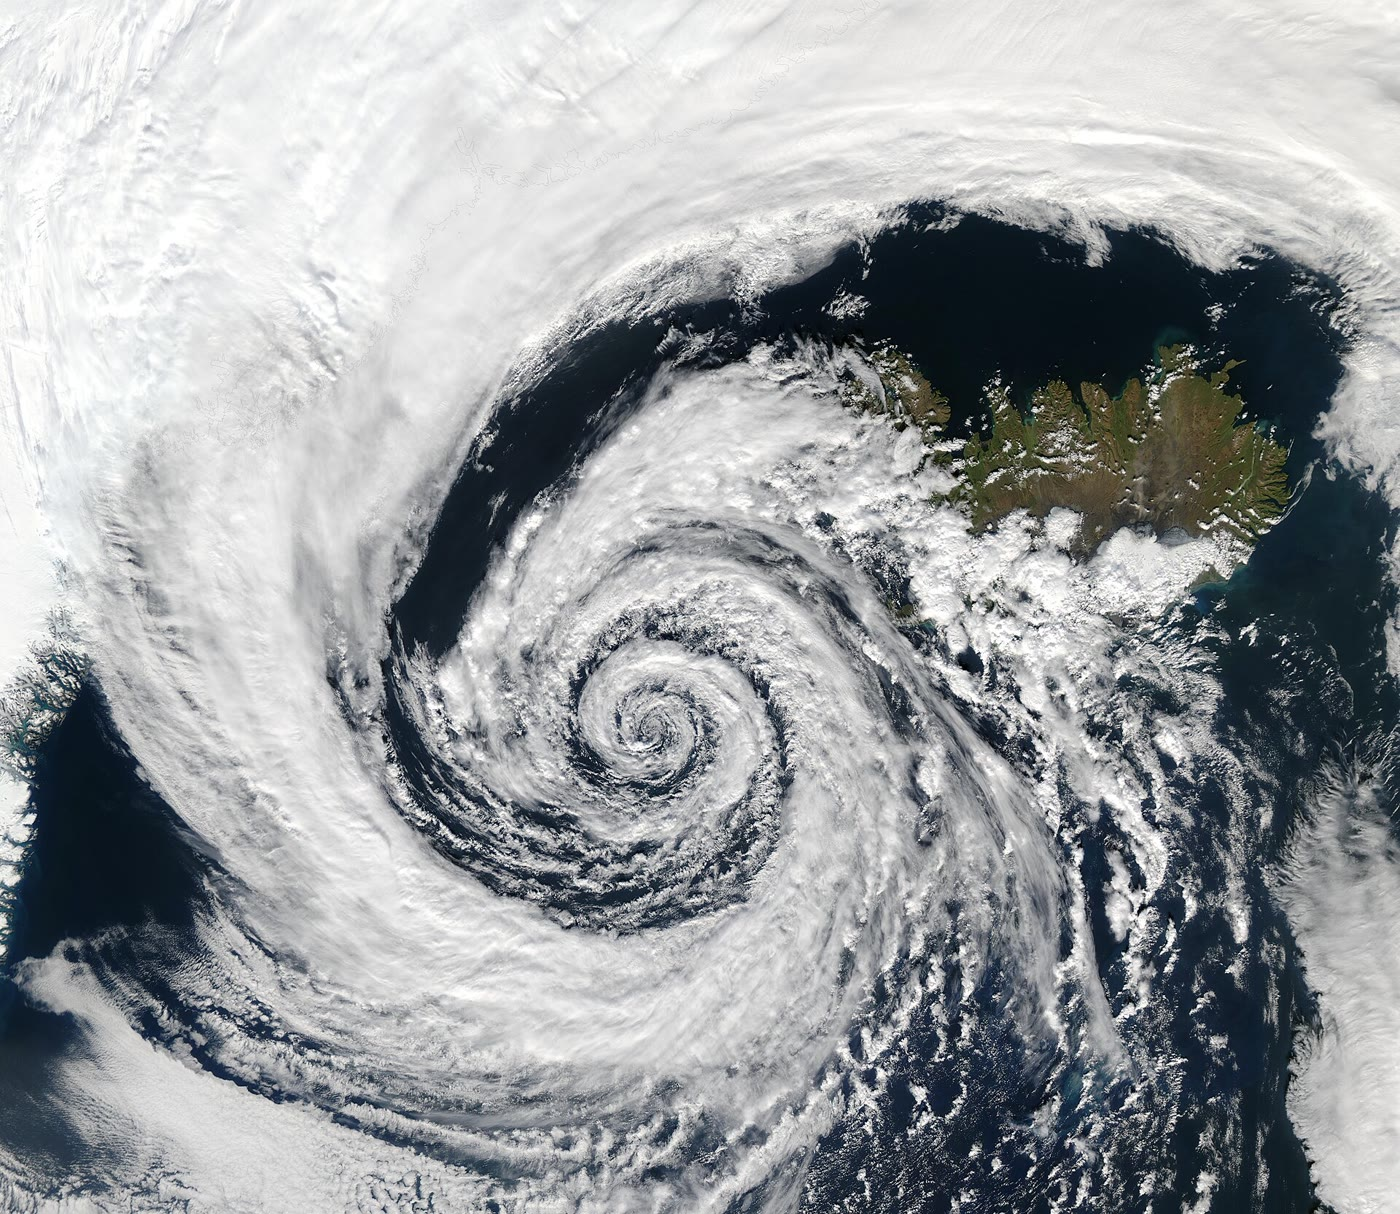
\includegraphics[width=\linewidth]{images/book5/b3-iceland-low.jpg}
\end{minipage}

\par\smallskip{\small Left, the Eady growth rate against wavelength for the
January zonal-mean shear at \ang{45} N (NCEP--NCAR Reanalysis~1,
1991--2020), the mean tropospheric stratification and $H = \qty{11}{km}$:
no growth below \qty{3200}{km}, fastest growth near \qty{4700}{km}. Right, a
depression in its mature stage off the south-west coast of Iceland, 4
September 2003, its clouds wound into an anticlockwise spiral round the
low (NASA/GSFC, MODIS Rapid Response Team, public
domain).}\label{fig:b3:atmospheric-dynamics:eady}
\end{omfigure}
% ledger: data:b5-ncep-uwnd, nasa:grc-atmos, photo:b3-iceland-low

The extratropical cyclone of the Year~2 volume is the surface face of a
growing \omterm{def:b3:gfd-foundations:baroclinic}{baroclinic} wave: its warm sector carries warm air poleward and
upward, the cold air behind it slides equatorward and down, and the trough
aloft tilts westward with height, as the release of \omterm{def:b3:atmospheric-dynamics:ape}{available potential
energy} requires.

\section{The general circulation}\label{sec:b3:atmospheric-dynamics:general-circulation}

The general circulation is described by averaging round latitude circles,
and what the average leaves out is as important as what it keeps.

\begin{definition}[Zonal mean and eddies]\label{def:b3:atmospheric-dynamics:eddy}
The \emph{zonal mean}\index{zonal mean} of a quantity $A$ is its average
round a latitude circle at fixed height or pressure, $[A] =
(1/2\pi)\int_0^{2\pi} A\,\mathrm d\lambda$. The departure $A^* = A - [A]$
is its eddy part; an \emph{eddy}\index{eddy (atmospheric)} of the
atmosphere is any departure of the flow from its zonal mean: travelling
waves, stationary waves, cyclones and anticyclones.
\end{definition}

The \omterm{def:b3:atmospheric-dynamics:eddy}{zonal mean} of a product splits in two: $[vT] = [v][T] + [v^*T^*]$. The
first term is the transport by the mean meridional circulation, the cells
of the Year~1 volume; the second the transport by the eddies. In the
middle latitudes the mean meridional wind is weak and the \omterm{def:b3:atmospheric-dynamics:eddy}{eddy} term
dominates: poleward-moving air is warmer than equatorward-moving air at the
same latitude, as in the figure below, and $[v^*T^*] > 0$. The eddies also
carry westerly momentum, $[u^*v^*]$, from the subtropics into the latitudes
of the jet, which is why the jet and the westerlies at the ground are
maintained against friction. The Ferrel cell of the Year~1 volume is the
mean meridional circulation that this \omterm{def:b3:atmospheric-dynamics:eddy}{eddy} transport forces.

\begin{omfigure}
\begin{tikzpicture}[>=stealth, font=\small, declare function={s(\x)=0.9*sin(\x r); t(\x)=0.9*sin((\x+1.0) r);}]
\draw[thick, black, domain=0:12.566, samples=120] plot (\x, {s(\x)});
\draw[omThm, thick, densely dashed, domain=0:12.566, samples=120] plot (\x, {t(\x)-0.15});
\foreach \x in {0.3, 6.58} {\draw[->, omThm, very thick] (\x,-1.1) -- (\x,1.15)
  node[above, font=\scriptsize] {warm};}
\foreach \x in {3.45, 9.73} {\draw[->, omDef, very thick] (\x,1.1) -- (\x,-1.15)
  node[below, font=\scriptsize] {cold};}
\node[font=\scriptsize, anchor=west] at (12.7,{s(12.566)}) {streamline};
\node[font=\scriptsize, anchor=west, omThm] at (12.7,{t(12.566)-0.15}) {isotherm};
\draw[->] (-1.6,-1.1) -- (-0.6,-1.1) node[below, font=\scriptsize] {east};
\draw[->] (-1.6,-1.1) -- (-1.6,-0.1) node[above, font=\scriptsize] {north};
\node[font=\scriptsize] at (6.3,-1.95) {cold air to the north, warm to the south};
\end{tikzpicture}

\par\smallskip{\small A growing \omterm{def:b3:gfd-foundations:baroclinic}{baroclinic} wave in plan view (schematic,
Northern Hemisphere, westerly flow). The isotherm (dashed) lags the
streamline by a quarter wavelength or less, so the air moving north (red
arrows) is warmer than the air moving south at the same latitude (blue):
the wave carries heat poleward, $[v^*T^*] >
0$.}\label{fig:b3:atmospheric-dynamics:heatflux}
\end{omfigure}

In the tropics the eddies are weak and the mean circulation carries heat
poleward, the Hadley cell. The Year~1 volume found that air leaving the
equator at rest and keeping its angular momentum would blow at hundreds of
metres per second at \ang{40}, and left open why the cell ends near
\ang{30}. A simple model answers.

\begin{definition}[Atmospheric angular momentum; Held--Hou model]\label{def:b3:atmospheric-dynamics:held-hou}
The \emph{atmospheric angular momentum}\index{atmospheric angular momentum}
per unit mass about the Earth's axis is $M = (\Omega a\cos\varphi +
u)\,a\cos\varphi$, for an eastward wind $u$ at latitude $\varphi$. The
\emph{Held--Hou model}\index{Held--Hou model} of the Hadley cell is an
axisymmetric, steady circulation of a dry Boussinesq atmosphere of depth
$H$, heated by relaxation towards a radiative-equilibrium potential
temperature $\theta_E/\theta_0 = 1 + \Delta/3 - \Delta\sin^2\varphi$; its
upper branch conserves $M$, its lower branch has negligible wind, and the
flow is in thermal-wind balance.
\end{definition}

\begin{theorem}[Extent of the Hadley cell]\label{thm:b3:atmospheric-dynamics:held-hou}
In the small-angle limit, the Held--Hou cell reaches the latitude
\[
\varphi_H = \left(\frac{5\,gH\Delta}{3\,\Omega^2a^2}\right)^{1/2}
\]
in each hemisphere, and the wind of its upper branch is $u_M = \Omega
a\varphi^2$.
\end{theorem}

\begin{proof}
At small $\varphi$, $\cos\varphi \approx 1$ and air leaving the equator at
rest with $M = \Omega a^2$ has $u_M = \Omega a(1 - \cos^2\varphi)/\cos\varphi
\approx \Omega a\varphi^2$. With $f \approx 2\Omega\varphi$, $y = a\varphi$,
no wind at the ground and the \omterm{thm:b3:gfd-foundations:thermal-wind}{thermal wind} in its Boussinesq form over the
depth $H$, $2\Omega\varphi\,u_M/H = -(g/a\theta_0)\,\partial\theta_M/
\partial\varphi$, where $\theta_M$ is the vertical mean of $\theta$ in the
cell. Then $\partial(\theta_M/\theta_0)/\partial\varphi = -2\Omega^2a^2
\varphi^3/(gH)$ and $\theta_M/\theta_0 = A - K\varphi^4$, $K = \Omega^2a^2/
(2gH)$. Inside the cell the circulation moves heat but neither creates nor
destroys it, so the cell has the same mean temperature as radiative
equilibrium: $\int_0^{\varphi_H}\theta_M\,\mathrm d\varphi = \int_0^{\varphi_H}
\theta_E\,\mathrm d\varphi$. At its edge the temperature is continuous:
$\theta_M(\varphi_H) = \theta_E(\varphi_H)$. With $\theta_E/\theta_0 \approx
B - \Delta\varphi^2$, $B = 1 + \Delta/3$, the first condition gives $A - B =
K\varphi_H^4/5 - \Delta\varphi_H^2/3$, the second $A - B = K\varphi_H^4 -
\Delta\varphi_H^2$. Subtracting, $(4/5)K\varphi_H^4 = (2/3)\Delta
\varphi_H^2$, so $\varphi_H^2 = 5\Delta/(6K) = 5gH\Delta/(3\Omega^2a^2)$.
\end{proof}

The cell ends where the temperature that angular-momentum conservation
imposes meets radiative equilibrium; beyond, the atmosphere would have to
be colder than radiation makes it. The model has two parameters that are
not observed directly. For $H = \qty{15}{km}$ and $\Delta$ between $1/6$ and
$1/3$, chosen for illustration, $\varphi_H$ is \ang{25} to \ang{35}. The
observed cells, read from the zonal-mean meridional wind, end at
\ang{33.3} N and \ang{32.5} S in the annual mean, and the winter cells,
the strong ones, at \ang{30.8} N in December--February and \ang{29.1} S in
June--August. The scaling is the point: a cell that widens with a
deeper troposphere and a stronger heating contrast, and narrows on a
faster-rotating planet. The model's upper wind, $u_M =
\qty{88}{m/s}$ at its edge for $\Delta = 1/6$, is twice the observed jet:
the eddies take the excess away.
% ledger: geod5:grs80-defining, earth:Rmean, data:b5-ncep-vwnd (values in figdata/bachelor-3/held_hou.py)

\begin{omfigure}
\begin{tikzpicture}
\begin{groupplot}[group style={group size=2 by 1, horizontal sep=1.7cm},
  width=0.48\linewidth, height=0.44\linewidth, tick label style={font=\scriptsize},
  label style={font=\small}, legend style={font=\scriptsize, draw=none, fill=none}]
\nextgroupplot[xlabel={latitude (\unit{\degree})}, ylabel={$100\,(\theta/\theta_0 - 1)$},
  xmin=0, xmax=60, ymin=-30, ymax=15, legend pos=south west, legend cell align=left,
  title={\small $\Delta = 1/3$, $H = \qty{15}{km}$}]
% computed in figdata/bachelor-3/held_hou.py
\addplot[omDef, thick] table[x=phi, y=thE] {figdata/out/bachelor-3-held_hou-theta-3.dat};
\addplot[omThm, thick, unbounded coords=jump] table[x=phi, y=thM] {figdata/out/bachelor-3-held_hou-theta-3.dat};
\addplot[black!50, densely dashed, forget plot] coordinates {(35.26,-30) (35.26,15)};
\node[font=\scriptsize, anchor=south west] at (axis cs:35.6,7) {$\varphi_H$};
\legend{$\theta_E$, $\theta_M$}
\nextgroupplot[xlabel={latitude (\unit{\degree})}, ylabel={$\psi$ at \qty{500}{hPa} ($10^{10}$\,\unit{kg/s})},
  xmin=-60, xmax=60, ymin=-25, ymax=25, xtick={-60,-30,0,30,60}, legend pos=south west,
  legend cell align=left]
\addplot[black!50, thin, domain=-60:60, samples=2, forget plot] {0};
\addplot[black, thick] table[x=lat, y=ann] {figdata/out/bachelor-3-held_hou-psi.dat};
\addplot[omDef, thick] table[x=lat, y=djf] {figdata/out/bachelor-3-held_hou-psi.dat};
\addplot[omThm, thick] table[x=lat, y=jja] {figdata/out/bachelor-3-held_hou-psi.dat};
\legend{year, Dec--Feb, Jun--Aug}
\end{groupplot}
\end{tikzpicture}

\par\smallskip{\small Left, the Held--Hou construction: the
angular-momentum-conserving temperature of the cell (red) meets radiative
equilibrium (blue) at $\varphi_H = \ang{35}$, with equal areas between the
curves inside the cell. Right, the mean meridional mass streamfunction at
\qty{500}{hPa} from the zonal-mean meridional wind (NCEP--NCAR
Reanalysis~1, 1991--2020; positive where the air above \qty{500}{hPa}
moves north): the strong
winter-hemisphere cell straddles the equator, and the cells end near
\ang{30}.}\label{fig:b3:atmospheric-dynamics:held-hou}
\end{omfigure}
% ledger: data:b5-ncep-vwnd

\begin{history}[From long waves to the first computed forecast]
In 1939 C.-G.~Rossby and his collaborators, in the \emph{Journal of Marine
Research}, set out to interpret several apparently independent phenomena
of the weather from a single point of view. Motivated by weather patterns
that move upstream against the prevailing westerly flow, Rossby wrote down
a linearised theory in which large-scale disturbances tend to move westward
and smaller ones eastward relative to the wind: the waves and the
$\beta$-plane of this chapter. Eleven years later J.~G.~Charney,
R.~Fjørtoft and J.~von~Neumann integrated the \omterm{thm:b3:atmospheric-dynamics:bve}{barotropic vorticity equation}
numerically on the electronic computer ENIAC: four forecasts of 24~hours at
the \qty{500}{mb} level, on a grid of \qty{736}{km}, 8 degrees of longitude
at \ang{45}. The computation of each forecast took about 24~hours: they
were, as they wrote, just able to keep pace with the weather.
\end{history}
% ledger: rossby39:paper, jmr20:commentary, charney50:eniac

\section{Exercises}

\begin{exercise}[$\star$]\label{exo:b3:atmospheric-dynamics:1}
(a)~Compute the \omterm{def:b3:atmospheric-dynamics:vorticity-kinds}{relative vorticity} of a vortex in solid rotation that turns
once a day. (b)~Compute the \omterm{def:b3:atmospheric-dynamics:vorticity-kinds}{planetary vorticity} at \ang{30} and \ang{60} N
($\Omega = \qty{7.292e-5}{rad/s}$) and compare.
\end{exercise}

\begin{exercise}[$\star$]\label{exo:b3:atmospheric-dynamics:2}
A parcel with no \omterm{def:b3:atmospheric-dynamics:vorticity-kinds}{relative vorticity} at \ang{30} N moves to \ang{40} N in a
flow without divergence. Compute its \omterm{def:b3:atmospheric-dynamics:vorticity-kinds}{relative vorticity} there. Is it
cyclonic or anticyclonic?
\end{exercise}

\begin{exercise}[$\star$]\label{exo:b3:atmospheric-dynamics:3}
At \ang{45} N, with no mean wind, compute the phase speed of a Rossby wave
of wavelength \qty{5000}{km} with $l = 0$. In which direction does it move?
\end{exercise}

\begin{exercise}[$\star$]\label{exo:b3:atmospheric-dynamics:4}
At \ang{60} N in a westerly of \qty{10}{m/s}, compute $\beta$, the
stationary wavelength and the number of stationary waves round the
latitude circle ($a = \qty{6371}{km}$).
\end{exercise}

\begin{exercise}[$\star\star$]\label{exo:b3:atmospheric-dynamics:5}
A column of air \qty{10}{km} deep, without \omterm{def:b3:atmospheric-dynamics:vorticity-kinds}{relative vorticity} at \ang{45}
N, crosses a mountain range that squeezes it to \qty{8}{km}, then a basin
where it is \qty{12}{km} deep. Assuming it stays near \ang{45} N, compute its
\omterm{def:b3:atmospheric-dynamics:vorticity-kinds}{relative vorticity} over the range and over the basin. Where will
depressions tend to form?
\end{exercise}

\begin{exercise}[$\star\star$]\label{exo:b3:atmospheric-dynamics:6}
For the wave with five crests round the \ang{45} N circle ($l = 0$) in a
westerly of \qty{15}{m/s}, compute the phase speed and the group velocity.
How long does the wave's energy take to travel \qty{5000}{km} east, and how
long the pattern?
\end{exercise}

\begin{exercise}[$\star\star$]\label{exo:b3:atmospheric-dynamics:7}
At \ang{45} N in a westerly of \qty{15}{m/s}, a wave is confined between
latitudes so that $l = \pi/(\qty{6000}{km})$. (a)~Compute its stationary
zonal wavenumber and wavelength. (b)~Show that no stationary wave exists for
$l = \pi/(\qty{3000}{km})$.
\end{exercise}

\begin{exercise}[$\star\star$]\label{exo:b3:atmospheric-dynamics:8}
In an \omterm{def:b3:atmospheric-dynamics:eady}{Eady model} at \ang{45} N, $\Lambda = \qty{2e-3}{s^{-1}}$, $N =
\qty{0.012}{s^{-1}}$ and $H = \qty{10}{km}$. Compute $L_d$, the growth rate
and $e$-folding time of the fastest-growing disturbance, and its
wavelength.
\end{exercise}

\begin{exercise}[$\star\star$]\label{exo:b3:atmospheric-dynamics:9}
Along a latitude circle the \omterm{def:b3:atmospheric-dynamics:eddy}{eddy} meridional wind is $v^* = V\cos kx$ and the
\omterm{def:b3:atmospheric-dynamics:eddy}{eddy} temperature $T^* = T_0\cos(kx - \delta)$, with $V = \qty{10}{m/s}$ and
$T_0 = \qty{5}{K}$. Compute $[v^*T^*]$ for $\delta = 0$, \ang{60} and
\ang{90}, and the corresponding heat flux $\rho c_p[v^*T^*]$ per
\unit{kg/m^3} of air ($c_p = \qty{1004}{J.kg^{-1}.K^{-1}}$). Which
arrangement transports no heat?
\end{exercise}

\begin{exercise}[$\star\star\star$]\label{exo:b3:atmospheric-dynamics:10}
Starting from the \omterm{thm:b3:atmospheric-dynamics:bve}{barotropic vorticity equation}, derive the dispersion
relation of Rossby waves in a uniform westerly, and show that relative to
the air every Rossby wave moves westward.
\end{exercise}

\begin{exercise}[$\star\star\star$]\label{exo:b3:atmospheric-dynamics:11}
In the \omterm{def:b3:atmospheric-dynamics:held-hou}{Held--Hou model} take $H = \qty{12}{km}$ and $\Delta = 1/4$. Compute
$\varphi_H$, the small-angle wind $u_M$ at the edge and the exact
angular-momentum wind there, and compare with the subtropical jet of
\qty{44}{m/s} of the January \omterm{def:b3:atmospheric-dynamics:eddy}{zonal mean}.
\end{exercise}

\begin{exercise}[$\star\star\star$]\label{exo:b3:atmospheric-dynamics:12}
Two layers of air differ in potential temperature by \qty{10}{K} on
\qty{300}{K}; their interface slopes upward towards the pole with slope $s$
across a band \qty{4000}{km} wide, and $\rho = \qty{0.7}{kg/m^3}$. (a)~Show
that letting the interface flatten releases $\rho g' s^2L^2/24$ per unit
area, $g' = g\,\Delta\theta/\theta$. (b)~Compute it for $s = 10^{-3}$ and
$2\times10^{-3}$ and compare with the kinetic energy of a \qty{15}{m/s}
wind through \qty{10}{km} of the same air.
\end{exercise}
% ledger: geod5:grs80-defining, earth:Rmean, data:b5-ncep-uwnd

\section{Problem: The Wave that Stood Still}

\begin{problem}[{Weekend problem --- vorticity, Rossby waves and the
growth of a \omterm{def:b3:gfd-foundations:baroclinic}{baroclinic} wave at \ang{45} N}]
\label{pb:b3:atmospheric-dynamics:1}
A westerly flow of \qty{15}{m/s} crosses the middle latitudes of an
invented continent, along \ang{45} N. Take $\Omega =
\qty{7.292115e-5}{rad/s}$, $a = \qty{6371}{km}$ and $g = \qty{9.81}{m/s^2}$.
All values of the flow are invented.

\medskip\noindent\textbf{Part I --- A displaced parcel.}
\begin{enumerate}
\item A parcel without \omterm{def:b3:atmospheric-dynamics:vorticity-kinds}{relative vorticity} at \ang{45} N is pushed to
  \ang{50} N. Compute $f$ at both latitudes and its \omterm{def:b3:atmospheric-dynamics:vorticity-kinds}{relative vorticity} at
  \ang{50} N, if the flow has no divergence.
\item Moving at \qty{15}{m/s}, along what radius of curvature does it turn
  (take $\zeta = -V/R$, all of it from curvature)? Which way does it turn?
\item If its column also shrinks from \qty{10.0}{km} to \qty{9.5}{km} on the
  way, what is its \omterm{def:b3:atmospheric-dynamics:vorticity-kinds}{relative vorticity} at \ang{50} N?
\item Pushed instead to \ang{40} N, without divergence, what \omterm{def:b3:atmospheric-dynamics:vorticity-kinds}{relative
  vorticity} does it acquire? Explain why a parcel displaced from its
  latitude oscillates about it.
\end{enumerate}

\medskip\noindent\textbf{Part II --- Travelling waves.}
\begin{enumerate}[resume]
\item Compute $\beta$ at \ang{45} N and the length of the latitude circle.
\item For $n = 3$ to 8 waves round the circle ($l = 0$), compute the
  wavelength, the phase speed and the group velocity in the westerly of
  \qty{15}{m/s}.
\item Which waves move west, which east? How many days does the wave
  $n = 5$ take to move \qty{1000}{km}?
\item A ridge over the west of the continent intensifies. Where, and after
  how long, will the effect of the wave $n = 6$ reach \qty{5000}{km}
  downstream?
\end{enumerate}

\medskip\noindent\textbf{Part III --- The wave that stood still.}
\begin{enumerate}[resume]
\item Compute the stationary wavelength and the stationary wavenumber at
  \ang{45} N.
\item Compute the stationary wavenumber for westerlies of 10 and
  \qty{20}{m/s}. What happens to the stationary waves when the westerlies
  strengthen in winter?
\item Compute the stationary wavenumber at \ang{35} N and \ang{55} N in the
  westerly of \qty{15}{m/s}.
\item The continent's western mountains rise \qty{2}{km} into a
  troposphere \qty{10}{km} deep. Compute the \omterm{def:b3:atmospheric-dynamics:vorticity-kinds}{relative vorticity} of a column
  that crosses them without changing latitude. Why do mountains force
  stationary waves?
\item Why does the wave pattern that the mountains force stand still
  only when its wavelength is near $\lambda_s$?
\end{enumerate}

\medskip\noindent\textbf{Part IV --- A storm grows.}
\begin{enumerate}[resume]
\item The westerly increases from the ground to \qty{10}{km} by
  \qty{25}{m/s}. Compute the shear $\Lambda$, and the poleward temperature
  gradient that it implies by the \omterm{thm:b3:gfd-foundations:thermal-wind}{thermal wind} at a mean temperature of
  \qty{250}{K}.
\item With $N = \qty{0.011}{s^{-1}}$, compute the Richardson number
  $N^2/\Lambda^2$. Is the flow unstable to small-scale shear turbulence?
\item Compute the Rossby radius $L_d$ for $H = \qty{10}{km}$.
\item Compute the wavelength of the fastest-growing Eady disturbance and
  the number of such waves round the latitude circle.
\item Compute the shortest wavelength that grows.
\item Compute the growth rate $\sigma_{\max}$.
\item By what factor does the disturbance grow in three days?
\item Compare the wavelength of the growing storm with the stationary
  wavelength of Part~III: which is longer, and what does that imply for the
  motion of the storms relative to the stationary waves?
\item Which way does the trough of the growing wave tilt with height, and
  why must it?
\item Give the $e$-folding time of the fastest-growing Eady disturbance.
\end{enumerate}
\end{problem}
% ledger: geod5:grs80-defining, earth:Rmean
